\section{Gewöhnliche Differentialgleichungen}

\begin{frame}{Erinnerung: Gewöhnliche Differentialgleichung}
    \begin{itemize}
        \item<1-> Eine \textbf{gewöhnliche Differentialgleichung erster Ordnung} hat die Form
        \begin{align}
            \label{ode-erste-ordnung}
            x^{\prime}(t) = f(t, x(t)),
        \end{align}
        wobei $f : D \times \mathbb{R}^{n} \rightarrow \mathbb{R}^{n}$ ist die \textit{rechte Seite}.
        \item<2-> Eine Lösung $x$ eines \textbf{Anfangswertproblem} erfüllt
        \begin{align}
            \label{awp-erste-ordnung}
            x^{\prime}(t) &= f(t, x(t)), \nonumber\\
            x(t_{0})&=x_{0}
        \end{align}
        mit zugehörigem Anfangswert $x_0 \in \mathbb{R}^n$.
        \item<3-> es gibt auch gewöhnliche Differentialgleichungen höherer Ordnung, die auf \eqref{ode-erste-ordnung}
        reduziert werden können.
    \end{itemize}
\end{frame}

\begin{frame}{Erinnerung: Existenz und Eindeutigkeit}
    \begin{itemize}
        \item<1-> Für eine stetige rechte Seite $f$ ist mit dem \textbf{Satz von Peano} die Existenz einer Lösung
        $x$ des Anfangswertproblems \eqref{awp-erste-ordnung} garantiert.
        \item<2-> Falls die rechte Seite $f$ stetig und Lipschitz-stetig im zweiten Argument ist, existiert nach
        dem \textbf{Satz von Picard-Lindelöf} eine eindeutige Lösung $x$.
        \begin{itemize}
            \item<1-> Für eine im zweiten Argument Lipschitz-stetige Funktion $f$ gilt dabei
            \[
                \left\lVert f(t,x) - f(t,y) \right\rVert_2 \leq L \left\lVert x -y \right\rVert_2
            \]
            für alle $(t,x), (t,y) \in \mathcal{M}$, wobei
            $\mathcal{M}\subset \mathbb{R} \times \mathbb{R}^n$.
        \end{itemize}
    \end{itemize}
\end{frame}

\begin{frame}{Erinnerung: Stetige Abhängigkeit der Daten}
    \begin{itemize}
        \item<1->  Für ein Anfangswertproblem \eqref{awp-erste-ordnung} mit Lipschitz-stetiger rechten Seite $f$ hängt
        die dazugehörige Lösung $x(t)$ für alle $t \in D \subset \mathbb{R}$ stetig von den Daten $(t_0,x_0, f)$ ab.
        \begin{itemize}
            \item Für obige Lösung $x$ und der stetig differenzierbaren Funktion $\hat{x}$ mit
            der Näherungslösung $(t,\hat{x}(t))$ gilt also unter den Voraussetzungen
            \begin{align*}
                \left\lVert \hat{x}^{\prime}(t) - f(t,\hat{x}(t)) \right\rVert_2 &\leq d_f \qquad t \in D,\\
                |t_{0} - \tilde{t}_0| &\leq d_t,\\
                \left\lVert x_0 - \hat{x}(\tilde{t}_0) \right\rVert_2 &\leq d_a,
            \end{align*}
            dass
            \[
                \left\lVert x(t) - \hat{x}(t) \right\rVert_2 \leq
                e^{L|t-t_0|}(d_a + d_t(d_f + \sup_{s \in D} \left\lVert f(s, \hat{x}(s)) \right\rVert_2)
                + \frac{d_f}{L}) - \frac{d_f}{L}.
            \]
        \end{itemize}
    \end{itemize}
\end{frame}

\begin{frame}{Beispiel: Abhängigkeit von den Daten}
    \begin{itemize}
        \item<1-> Gegebenes Anfangswertproblem
        \begin{align}
            \label{abhängigkeit-beispiel}
            x^{\prime} &= 10\left( x - \frac{t^2}{1 + t^2} \right) + \frac{2t}{(1+t^2)^2}, \nonumber\\
            x(0)&=x_0
        \end{align}
        mit stetiger und im zweiten Argument Lipschitz-stetiger rechten Seite $f$.
        \item<2-> Wegen der speziellen Form $x^{\prime}(t)=Ax(t) +b (t)$ des Anfangswertproblems
        \eqref{abhängigkeit-beispiel} kann die eindeutige Lösung explizit angegeben werden:
        \[
            x(t) = x_0e^{10t} + \frac{t^2}{1+t^2}
        \]
    \end{itemize}
\end{frame}

\begin{frame}{Beispiel: Abhängigkeit von den Daten}
    \begin{itemize}
        \item<1-> Für den Anfangswert $x_0=0$ hat \eqref{abhängigkeit-beispiel} die Lösung
        $x(t)=\frac{t^2}{(1+t^2)}$.
        \item<1-> Für den gestörten Anfangswert $\hat{x}_0=-10^{-10}$ hat \eqref{abhängigkeit-beispiel} die Lösung
        $\hat{x}(t)=-10^{-10}e^{10t} + \frac{t^2}{(1+t^2)}$.
        \item<2-> Kleiner Fehler in den Anfangsdaten $|x_0 - \hat{x}_0| = 1ß^{-10}$ vorliegen.
    \end{itemize}
\end{frame}

\begin{frame}{Beispiel: Abhängigkeit von den Daten}
    \begin{figure}
        \begin{center}
            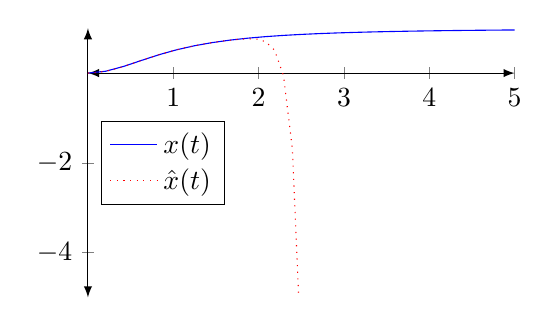
\begin{tikzpicture}
                \begin{axis}[
                height=5cm,
                width=7cm,
                ymin=-5, ymax=1,
                axis lines=middle,
                axis line style={latex-latex},
                legend style={at={(0.03,0.5)},anchor=west}
                ]
                \addplot[domain = 0:5,blue] {(x^2)/(1+x^2)};
                \addplot[dotted, domain = 0:2.5,red] {(-10^(-10))*exp(10*x) + (x^2)/(1+x^2)};
                \legend{
                    $x(t)$,
                    $\hat{x}(t)$
                }
                \end{axis}
            \end{tikzpicture}
            \caption{Lösungen $x(t)$ und $\hat{x}(t)$.}
            \label{sigmoid-figure}
        \end{center}
    \end{figure}
    \begin{itemize}
        \item<1-> Für hinreichend große $t$ führt ein geringer Fehler der Anfangswerten jedoch zu einem großen
        Fehler der Lösungen $|x(t) - \hat{x}(t)|=10^{-10}e^{10t}$.
    \end{itemize}
\end{frame}